\chapter{O exercício e as necessidades energéticas do corpo}\label{ch:g10:exercise-and-energy}

Uma ciclista numa bicicleta de laboratório pedala contra um freio que
mede a potência dela: \qty{100}{W}, depois \qty{150}{W}, depois
\qty{200}{W}. Uma máscara sobre o rosto dela manda cada respiração para
um analisador. Os números da tela sobem no mesmo passo que o freio:
quanto mais trabalho mecânico ela entrega, mais oxigênio consome e mais
gás carbônico expira. Os músculos dela estão fazendo a respiração do
\cref{ch:g10:cell-metabolism} a todo vapor, e o analisador está lendo o
balanço disso. Este capítulo acompanha a energia do exercício, do
alimento que a fornece ao oxigênio que a libera.

\section{Energia que entra, trabalho que sai}

\begin{definition}[Gasto energético]\label{def:g10:exercise-and-energy:expenditure}
O \emph{gasto energético}\index{gasto energético} do corpo, em joules,
é a energia total que as \omterm{def:g10:cells-common-unit:cell}{células} dele liberam de moléculas orgânicas ao
longo de um dado tempo. Dividido pelo tempo, ele é uma
\emph{potência metabólica}, em watts. Em repouso, um adulto gasta cerca
de \qty{80}{W} --- uns \qty{7000}{kJ} por dia --- para manter o coração
batendo, o cérebro funcionando, a temperatura a \qty{37}{\celsius} e as
\omterm{def:g10:cells-common-unit:cell}{células} vivas; é o \emph{\omterm{def:g10:cell-metabolism:metabolism}{metabolismo} basal}. Toda atividade se soma a
ele.
\end{definition}

\begin{proposition}[Para onde vai a energia]\label{prop:g10:exercise-and-energy:efficiency}
Um músculo em atividade converte só cerca de um quarto da energia que
libera em trabalho mecânico; os outros três quartos saem como calor.
Entregar uma potência mecânica $P$ custa portanto ao corpo uma
potência metabólica de cerca de $4P$ acima do repouso: uma ciclista a
\qty{100}{W} nos pedais está gastando uns \qty{400}{W} nos músculos, e
o corpo dela precisa se livrar de \qty{300}{W} de calor --- suando,
principalmente.
\end{proposition}
\admitted

\begin{example}[Orçamentos diários]\label{ex:g10:exercise-and-energy:budgets}
Um estudante sentado na aula, andando até a escola e dormindo gasta
cerca de \qty{9000}{kJ} por dia; uma hora de futebol acrescenta uns
\qty{2500}{kJ}; um dia na montanha com mochila, \qty{15000}{kJ} ao
todo. Um ciclista numa etapa de montanha de uma corrida gasta
\qty{25000}{kJ}, e não consegue comer o bastante durante o dia para
cobrir isso. A energia vem do alimento
(\cref{ch:g10:chemistry-of-life}): \qty{17}{kJ} por grama de
\omterm{def:g10:chemistry-of-life:families}{carboidrato} ou de \omterm{def:g10:chemistry-of-life:families}{proteína}, \qty{38}{kJ} por grama de \omterm{def:g10:chemistry-of-life:families}{lipídio}.
\end{example}

\section{O consumo de oxigênio mede o gasto energético}

\begin{proposition}[O equivalente energético do oxigênio]\label{prop:g10:exercise-and-energy:oxygen}
Como a energia do exercício é liberada pela \omterm{prop:g10:cell-metabolism:respiration}{respiração celular}, que
consome oxigênio, o consumo de oxigênio do corpo mede o \omterm{def:g10:exercise-and-energy:expenditure}{gasto
energético} dele: cada litro de oxigênio consumido corresponde a cerca
de \qty{20}{kJ} liberados, seja qual for a mistura de glicose e de
\omterm{def:g10:chemistry-of-life:families}{lipídios} queimada. Em repouso uma pessoa consome cerca de
\qty{0.25}{L} de oxigênio por minuto; durante o exercício o consumo
sobe em proporção à potência entregue, até um teto pessoal.
\end{proposition}
\begin{proof}[Evidências]
A equação da respiração do \cref{ch:g10:cell-metabolism} dá
\qty{2870}{kJ} para \qty{6}{mol} de oxigênio, ou seja \qty{478}{kJ} por
mol, e um mol de gás ocupa cerca de \qty{24}{L}: \qty{20}{kJ} por
litro. Para os \omterm{def:g10:chemistry-of-life:families}{lipídios} o número é \qty{19.6}{kJ/L}, para os
\omterm{def:g10:chemistry-of-life:families}{carboidratos} \qty{21.1}{kJ/L}, de modo que a mistura quase não importa.
Medidas em câmaras fechadas, em que o calor liberado por um sujeito é
recolhido diretamente, concordam com o número do oxigênio a menos de
alguns por cento.
\end{proof}

\begin{omfigure}
\begin{tikzpicture}
\begin{axis}[
  width=0.86\linewidth, height=5.8cm,
  axis x line=bottom, axis y line=left,
  xmin=0, xmax=320, ymin=0, ymax=4.2,
  xlabel={potência mecânica (W)}, ylabel={$\mathrm{O_2}$ consumido (L/min)},
  xlabel style={font=\small, at={(axis description cs:0.5,-0.12)}, anchor=north},
  ylabel style={font=\small},
  tick label style={font=\small},
  xtick={0,50,100,150,200,250,300}, ytick={0,1,2,3,4},
  clip=false,
]
\addplot[thick, omThm, mark=*, mark size=1.6pt] coordinates
  {(0,0.3) (50,0.9) (100,1.5) (150,2.1) (200,2.7) (250,3.2) (300,3.3)};
\draw[dashed, gray] (axis cs:0,3.3) -- (axis cs:320,3.3);
\node[font=\small, anchor=south east] at (axis cs:318,3.32) {$\dot V\!\mathrm{O_2}$max};
\node[font=\small, anchor=south west, align=left] at (axis cs:40,3.42) {inclinação: \qty{12}{mL} de $\mathrm{O_2}$ por minuto\\ para cada watt};
\end{axis}
\end{tikzpicture}

{\small Consumo de oxigênio de um sujeito pedalando em potência
crescente. A subida é linear --- cerca de \qty{12}{mL} de oxigênio por
minuto por watt --- até o consumo alcançar o teto dele, o
$\dot V\!\mathrm{O_2}$max do sujeito; além dele, a potência extra é
fornecida sem oxigênio e não pode ser sustentada.}
\end{omfigure}

\begin{definition}[Consumo máximo de oxigênio]\label{def:g10:exercise-and-energy:vo2max}
O \emph{consumo máximo de oxigênio}\index{consumo máximo de oxigênio},
escrito $\dot V\!\mathrm{O_2}$max, é a maior taxa com que o corpo de
uma pessoa consegue captar e usar oxigênio, em litros por minuto ---
ou, para comparar pessoas de tamanhos diferentes, em mililitros por
minuto por quilograma de massa corporal. Ele fixa a maior potência que
pode ser sustentada só pela respiração. Valores típicos:
\qty{35}{mL/min} por quilograma num adulto sedentário, \num{50} num
estudante treinado, \num{80} ou mais num campeão de provas de
resistência.
\end{definition}

\begin{example}[Ler a curva]\label{ex:g10:exercise-and-energy:reading}
Na figura, pedalar a \qty{100}{W} custa \qty{1.5}{L/min} de oxigênio:
$1.5 \times 20 = \qty{30}{kJ}$ por minuto, ou seja \qty{500}{W} de
potência metabólica --- os \qty{100}{W} de trabalho mais \qty{400}{W} de
calor e de necessidades de repouso, de acordo com a
\cref{prop:g10:exercise-and-energy:efficiency}. O teto de
\qty{3.3}{L/min} para um sujeito de \qty{66}{kg} são \qty{50}{mL/min}
por quilograma.
\end{example}

\begin{omfigure}
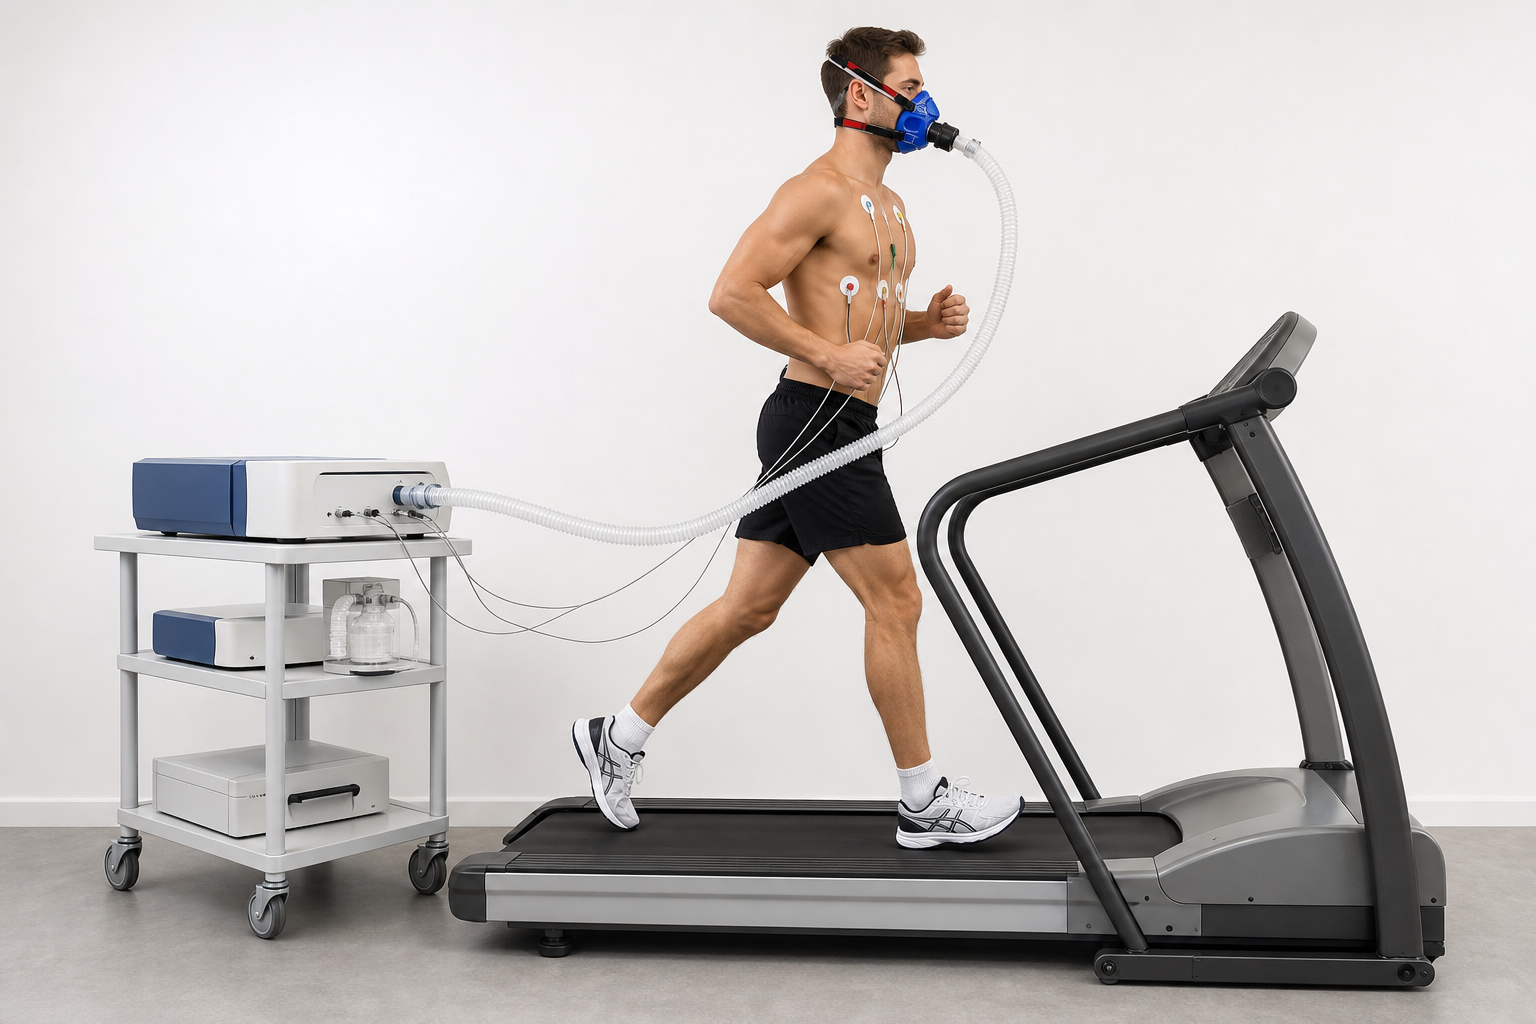
\includegraphics[width=0.62\linewidth]{images/book2/ai/g10-exercise-treadmill-mask.png}

{\small Medir o consumo de oxigênio durante o exercício: cada
respiração passa pela máscara até um analisador de gases que registra o
oxigênio captado e o gás carbônico liberado, minuto a minuto, enquanto
a esteira fixa a potência.}
\end{omfigure}

\section{Os combustíveis do músculo}

\begin{proposition}[Três fontes de ATP]\label{prop:g10:exercise-and-energy:fuels}
A contração muscular é paga em ATP, e a \omterm{def:g10:cells-common-unit:cell}{célula} guarda apenas alguns
segundos de reserva dele. Ele é renovado por três vias, cada uma com
velocidade e capacidade próprias:
\begin{itemize}
  \item uma pequena reserva de um composto fosfatado no músculo, que
        refaz o ATP instantaneamente mas dura cerca de dez segundos ---
        o tiro curto;
  \item a \omterm{def:g10:cell-metabolism:fermentation}{fermentação} láctica da glicose no \omterm{def:g10:cells-common-unit:cell}{citoplasma}, rápida mas
        perdulária, que sustenta um esforço máximo por um a dois
        minutos e produz ácido láctico;
  \item a \omterm{prop:g10:cell-metabolism:respiration}{respiração celular} nas \omterm{def:g10:cells-common-unit:organelle}{mitocôndrias}, mais lenta para chegar
        ao ritmo máximo mas de duração quase ilimitada, queimando
        glicose do sangue, \omterm{def:g10:exercise-and-energy:glycogen}{glicogênio} do músculo e ácidos graxos da
        gordura do corpo.
\end{itemize}
A parcela de cada uma depende da intensidade e da duração do
exercício.
\end{proposition}
\admitted

\begin{omfigure}
\begin{tikzpicture}
\begin{axis}[
  ybar stacked, bar width=18pt,
  width=0.86\linewidth, height=5.6cm,
  axis x line=bottom, axis y line=left,
  ymin=0, ymax=100, ylabel={parcela da energia (\%)}, ylabel style={font=\small},
  symbolic x coords={10 s, 1 min, 4 min, 30 min, 2 h},
  xtick=data, tick label style={font=\small},
  xlabel={duração de um esforço máximo},
  xlabel style={font=\small, at={(axis description cs:0.5,-0.12)}, anchor=north},
  enlarge x limits=0.15,
  legend style={at={(0.5,-0.3)}, anchor=north, legend columns=3,
                font=\small, draw=none},
]
\addplot[fill=omThm!50, draw=omThm] coordinates {(10 s,85) (1 min,25) (4 min,8) (30 min,2) (2 h,1)};
\addplot[fill=omProp!50, draw=omProp] coordinates {(10 s,12) (1 min,50) (4 min,32) (30 min,8) (2 h,2)};
\addplot[fill=omDef!50, draw=omDef] coordinates {(10 s,3) (1 min,25) (4 min,60) (30 min,90) (2 h,97)};
\legend{reserva de fosfato, fermentação láctica, respiração}
\end{axis}
\end{tikzpicture}

{\small Parcela aproximada das três fontes de ATP num esforço máximo de
dada duração. Um tiro de 100 metros funciona com a reserva de fosfato;
uma prova de 400 metros, em boa parte com a \omterm{def:g10:cell-metabolism:fermentation}{fermentação}; qualquer coisa
além de alguns minutos, com a respiração.}
\end{omfigure}

\begin{definition}[Glicogênio]\label{def:g10:exercise-and-energy:glycogen}
O \emph{glicogênio}\index{glicogênio} é a forma animal de \omterm{def:g10:chemistry-of-life:families}{carboidrato}
armazenado: uma cadeia ramificada de unidades de glicose, mantida como
grânulos nas \omterm{def:g10:cells-common-unit:cell}{células} musculares (cerca de \qty{400}{g} num adulto) e no
fígado (cerca de \qty{100}{g}). O glicogênio muscular abastece o
músculo que o armazena; o glicogênio do fígado é degradado em glicose
liberada no sangue, mantendo a glicose sanguínea perto de \qty{1}{g/L}
para o cérebro e os demais tecidos. A gordura, armazenada nas \omterm{def:g10:cells-common-unit:cell}{células}
adiposas, é a reserva bem maior (\cref{ch:g10:chemistry-of-life}), mas
só pode ser queimada devagar e só com oxigênio.
\end{definition}

\begin{example}[O muro da maratona]\label{ex:g10:exercise-and-energy:wall}
Correr consome cerca de \qty{4}{kJ} por quilograma de massa corporal
por quilômetro; um corredor de \qty{70}{kg} gasta \qty{280}{kJ/km}, e
uma maratona custa \qty{11800}{kJ}. As reservas de \omterm{def:g10:exercise-and-energy:glycogen}{glicogênio} guardam
cerca de \qty{8500}{kJ}. Se o corredor queimar \omterm{def:g10:exercise-and-energy:glycogen}{glicogênio} depressa
demais, as reservas acabam por volta do trigésimo quilômetro; os
músculos precisam então contar com a gordura, que fornece energia a
pouco mais da metade da taxa, e o ritmo desaba --- é ``bater no muro''.
Corredores treinados queimam uma parcela maior de gordura desde o
início, e comem \omterm{def:g10:chemistry-of-life:families}{carboidrato} durante a prova.
\end{example}

\begin{omfigure}
\begin{tikzpicture}[>=Stealth, font=\small,
  b/.style={draw, rounded corners, align=center, minimum height=0.9cm, text width=2.5cm}]
  \node[b, fill=omDef!12] (food) at (0,2.2) {alimento:\\ carboidratos, lipídios};
  \node[b, fill=omDef!12] (gly) at (0,0.6) {glicogênio (músculo,\\ fígado), glicose do sangue};
  \node[b, fill=omDef!12] (fat) at (0,-1.0) {ácidos graxos\\ da gordura do corpo};
  \node[b, fill=omThm!12, minimum height=2.6cm] (mit) at (4.3,-0.2) {mitocôndrias:\\ respiração};
  \node[b, fill=omProp!15] (o2) at (4.3,2.2) {oxigênio, dos\\ pulmões e do sangue};
  \node[b, fill=omMeth!15] (atp) at (9.2,-0.2) {ATP};
  \node[b, fill=white] (work) at (12.5,0.8) {trabalho muscular\\ (cerca de 25\%)};
  \node[b, fill=white] (heat) at (12.5,-1.2) {calor\\ (cerca de 75\%)};
  \draw[->] (food) -- (gly);
  \draw[->] (food.west) to[bend right=40] (fat.west);
  \draw[->] (gly) -- (mit);
  \draw[->] (fat) -- (mit);
  \draw[->] (o2) -- (mit);
  \draw[->] (mit) -- node[above, font=\scriptsize] {$\mathrm{CO_2}$ que sai} (atp);
  \draw[->] (atp) -- (work);
  \draw[->] (atp) -- (heat);
\end{tikzpicture}

{\small A cadeia energética do exercício prolongado: combustíveis do
alimento e das reservas do corpo, oxigênio da respiração pulmonar, ATP
fabricado nas \omterm{def:g10:cells-common-unit:organelle}{mitocôndrias} e gasto na contração --- com três quartos
dele saindo como calor.}
\end{omfigure}

\section{Medir e raciocinar}

\begin{method}[Um cálculo energético para o exercício]\label{met:g10:exercise-and-energy:calc}
\begin{enumerate}
  \item A partir do oxigênio: energia (\unit{kJ}) $=$ oxigênio
        consumido (\unit{L}) $\times 20$. Subtraia o consumo de repouso
        se a questão pedir o custo do exercício sozinho.
  \item A partir da potência mecânica: potência metabólica
        $\approx 4 P$; energia $=$ potência $\times$ tempo
        (\qty{1}{W} durante \qty{1}{s} é \qty{1}{J};
        \qty{1}{kWh} $= \qty{3600}{kJ}$).
  \item A partir do combustível: massa queimada $=$ energia $/$ valor
        energético (\qty{17}{kJ/g} para o \omterm{def:g10:chemistry-of-life:families}{carboidrato}, \qty{38}{kJ/g}
        para o \omterm{def:g10:chemistry-of-life:families}{lipídio}); o \omterm{def:g10:exercise-and-energy:glycogen}{glicogênio} é armazenado com três vezes a
        massa dele em água.
  \item Confira as ordens de grandeza: um dia inteiro são cerca de
        \qty{10000}{kJ}; uma hora puxada, \qtyrange{2000}{3000}{kJ};
        uma maratona, \qty{12000}{kJ}.
\end{enumerate}
\end{method}

\begin{example}[Uma hora de bicicleta]\label{ex:g10:exercise-and-energy:hour}
Uma hora a \qty{150}{W} nos pedais: potência metabólica de cerca de
\qty{600}{W}, energia $600 \times 3600 = \qty{2.16e6}{J} \approx
\qty{2200}{kJ}$; oxigênio $2200/20 = \qty{110}{L}$, ou seja
\qty{1.8}{L/min} --- coerente com a curva. Se metade vier do
\omterm{def:g10:chemistry-of-life:families}{carboidrato}: $1100/17 \approx \qty{65}{g}$ de glicose ou de
\omterm{def:g10:exercise-and-energy:glycogen}{glicogênio}, e $1100/38 \approx \qty{29}{g}$ de gordura.
\end{example}

\begin{remark}[Por que o oxigênio precisa chegar]\label{rem:g10:exercise-and-energy:delivery}
Tudo o que vem acima supõe que o oxigênio chegue às \omterm{def:g10:cells-common-unit:organelle}{mitocôndrias} tão
depressa quanto elas conseguem usá-lo. Esse é o trabalho dos pulmões,
do coração e do sangue, cuja resposta ao exercício --- respiração mais
rápida, batimento mais rápido e mais forte, sangue redirecionado aos
músculos --- é assunto do \cref{ch:g10:heart-lungs-effort}. O
$\dot V\!\mathrm{O_2}$max é sobretudo um limite de entrega, e não do
apetite dos músculos.
\end{remark}

\section{Exercícios}

\begin{exercise}[$\star$]\label{exo:g10:exercise-and-energy:1}
Defina \omterm{def:g10:cell-metabolism:metabolism}{metabolismo} basal e dê a ordem de grandeza dele em watts e em
quilojoules por dia.
\end{exercise}

\begin{exercise}[$\star$]\label{exo:g10:exercise-and-energy:2}
Uma pessoa consome \qty{2.0}{L} de oxigênio por minuto. Qual é o \omterm{def:g10:exercise-and-energy:expenditure}{gasto
energético} dela em quilojoules por minuto, e em watts?
\end{exercise}

\begin{exercise}[$\star$]\label{exo:g10:exercise-and-energy:3}
Cite as três vias pelas quais um músculo renova o ATP dele e dê a
duração típica que cada uma consegue sustentar sozinha.
\end{exercise}

\begin{exercise}[$\star$]\label{exo:g10:exercise-and-energy:4}
O que é o $\dot V\!\mathrm{O_2}$max? Converta \qty{3.5}{L/min} para um
sujeito de \qty{70}{kg} em mililitros por minuto por quilograma.
\end{exercise}

\begin{exercise}[$\star$]\label{exo:g10:exercise-and-energy:5}
Onde o \omterm{def:g10:exercise-and-energy:glycogen}{glicogênio} é armazenado, em que quantidades, e para que serve
cada reserva?
\end{exercise}

\begin{exercise}[$\star\star$]\label{exo:g10:exercise-and-energy:6}
Na figura do oxigênio em função da potência, leia o consumo de oxigênio
a \qty{200}{W} e calcule a potência metabólica. Deduza o calor
produzido por segundo.
\end{exercise}

\begin{exercise}[$\star\star$]\label{exo:g10:exercise-and-energy:7}
Uma caminhante de \qty{60}{kg} sobe \qty{800}{m} em duas horas.
Calcule o trabalho mecânico contra a gravidade
($g = \qty{9.8}{N/kg}$), a energia que os músculos dela gastaram se o
rendimento é de 25\%, e a potência metabólica média acima do repouso.
\end{exercise}

\begin{exercise}[$\star\star$]\label{exo:g10:exercise-and-energy:8}
Usando a figura das barras empilhadas, explique por que um corredor de
400 metros chega ofegante e dolorido enquanto um velocista de 100
metros mal está com a respiração acelerada.
\end{exercise}

\begin{exercise}[$\star\star$]\label{exo:g10:exercise-and-energy:9}
Uma atleta gasta \qty{3000}{kJ} numa sessão de treino, 60\% vindos de
\omterm{def:g10:chemistry-of-life:families}{carboidratos}. Que massa de \omterm{def:g10:exercise-and-energy:glycogen}{glicogênio} ela usou, e que massa de água foi
liberada junto?
\end{exercise}

\begin{exercise}[$\star\star$]\label{exo:g10:exercise-and-energy:10}
Uma barra de chocolate de \qty{50}{g} fornece \qty{1100}{kJ}. Por
quanto tempo ela alimentaria um ciclista pedalando a \qty{150}{W}?
\end{exercise}

\begin{exercise}[$\star\star$]\label{exo:g10:exercise-and-energy:11}
Por que a temperatura do corpo de uma pessoa sobe durante o exercício,
e por que mecanismo ela é impedida de subir mais?
\end{exercise}

\begin{exercise}[$\star\star\star$]\label{exo:g10:exercise-and-energy:12}
Dois sujeitos de \qty{60}{kg} e de \qty{90}{kg} têm ambos um
$\dot V\!\mathrm{O_2}$max de \qty{3.6}{L/min}. Qual dos dois consegue
correr mais rápido subindo um morro, e qual consegue pedalar mais
forte numa bicicleta de laboratório em terreno plano? Explique.
\end{exercise}

\begin{exercise}[$\star\star\star$]\label{exo:g10:exercise-and-energy:13}
O consumo de oxigênio de um corredor durante uma prova é de
\qty{3.0}{L/min} num ritmo que, pela curva, exigiria \qty{3.4}{L/min}.
De onde vem a diferença, e o que o corredor vai sentir depois de alguns
minutos?
\end{exercise}

\begin{exercise}[$\star\star\star$]\label{exo:g10:exercise-and-energy:14}
Explique por que uma pessoa não consegue perder gordura fazendo
exercício de intensidade máxima em tiros curtos com a mesma eficácia
com que a perde fazendo exercício moderado por muito tempo, usando as
três vias do ATP.
\end{exercise}

\begin{exercise}[$\star\star\star$]\label{exo:g10:exercise-and-energy:15}
Uma ciclista numa etapa de montanha gasta \qty{25000}{kJ} num dia. O
\omterm{def:g10:exercise-and-energy:glycogen}{glicogênio} dela guarda \qty{8500}{kJ} e ela come \qty{6000}{kJ} durante
a etapa. Estime a massa de gordura corporal que ela queima, e explique
por que os ciclistas comem sem parar numa etapa dessas.
\end{exercise}

\section{Problema: onde fica o muro}

\begin{problem}[{Problema de fim de semana --- o orçamento energético de
uma maratona: o oxigênio que a corredora respira, o glicogênio que ela
carrega, o quilômetro em que ele acaba, e o que o treino muda}]
\label{pb:g10:exercise-and-energy:1}
Nádia, de \qty{60}{kg}, corre uma maratona (\qty{42.2}{km}) em
\qty{3}{h}\,\qty{30}{min}. Correr custa \qty{4.0}{kJ} por quilograma
por quilômetro. Os músculos dela guardam \qty{300}{g} de \omterm{def:g10:exercise-and-energy:glycogen}{glicogênio} e o
fígado dela \qty{80}{g}; o \omterm{def:g10:exercise-and-energy:glycogen}{glicogênio} e a glicose dão \qty{17}{kJ/g}, a
gordura \qty{38}{kJ/g}; um litro de oxigênio libera \qty{20}{kJ}. O
$\dot V\!\mathrm{O_2}$max dela é de \qty{52}{mL/min} por quilograma.

\medskip
\noindent\textbf{Parte I --- O custo da prova.}
\begin{enumerate}
  \item Calcule o custo energético da maratona para Nádia.
  \item Calcule a potência metabólica média dela durante a prova, em
        watts.
  \item Calcule o volume de oxigênio que ela consome ao longo da prova,
        depois o consumo médio de oxigênio dela em litros por minuto.
  \item Expresse esse consumo em mililitros por minuto por quilograma,
        e como porcentagem do $\dot V\!\mathrm{O_2}$max dela.
  \item O consumo de repouso dela é de \qty{0.2}{L/min}. Que fração do
        consumo dela no dia da prova a corrida em si responde?
\end{enumerate}

\medskip
\noindent\textbf{Parte II --- As reservas.}
\begin{enumerate}[resume]
  \item Calcule a energia guardada nas reservas de \omterm{def:g10:exercise-and-energy:glycogen}{glicogênio} dela.
  \item Se ela queimasse apenas \omterm{def:g10:exercise-and-energy:glycogen}{glicogênio}, em que quilômetro as
        reservas acabariam?
  \item Na realidade ela queima uma mistura: 80\% de \omterm{def:g10:chemistry-of-life:families}{carboidrato}, 20\%
        de gordura no ritmo de prova dela. Em que quilômetro o
        \omterm{def:g10:exercise-and-energy:glycogen}{glicogênio} acaba agora?
  \item Que massa de gordura ela queima na prova? Compare com os
        \qty{9}{kg} de gordura que uma mulher de \qty{60}{kg}
        tipicamente carrega.
  \item Explique, a partir da
        \cref{prop:g10:exercise-and-energy:fuels}, por que ela não pode
        simplesmente queimar só gordura assim que o \omterm{def:g10:exercise-and-energy:glycogen}{glicogênio} acabar e
        manter o mesmo ritmo.
\end{enumerate}

\medskip
\noindent\textbf{Parte III --- Vencer o muro.}
\begin{enumerate}[resume]
  \item Durante a prova ela bebe uma solução açucarada que fornece
        \qty{60}{g} de \omterm{def:g10:chemistry-of-life:families}{carboidrato} por hora. Quanta energia isso
        acrescenta ao longo da prova, e quantos quilômetros de consumo
        de \omterm{def:g10:chemistry-of-life:families}{carboidrato} isso cobre?
  \item Refaça a questão 8 com a bebida. Ela agora termina antes de o
        \omterm{def:g10:exercise-and-energy:glycogen}{glicogênio} acabar?
  \item Três dias antes da prova ela faz uma ``carga'' de \omterm{def:g10:chemistry-of-life:families}{carboidrato},
        elevando o \omterm{def:g10:exercise-and-energy:glycogen}{glicogênio} muscular dela a \qty{500}{g}. Cada grama
        é armazenado com \qty{3}{g} de água. Quanto a massa dela sobe,
        e qual é o custo disso em energia por quilômetro?
  \item O treino desloca a mistura no ritmo de prova dela para 55\% de
        \omterm{def:g10:chemistry-of-life:families}{carboidrato} e 45\% de gordura. Com a carga e a bebida, em que
        quilômetro o \omterm{def:g10:exercise-and-energy:glycogen}{glicogênio} acabaria? Comente.
  \item Por que o cérebro, que usa apenas glicose, faz com que o
        esgotamento do \omterm{def:g10:exercise-and-energy:glycogen}{glicogênio} pareça exaustão mesmo quando os
        músculos ainda têm gordura para queimar?
\end{enumerate}

\medskip
\noindent\textbf{Parte IV --- Os números de um campeão.}
Um corredor de elite de \qty{55}{kg} corre a maratona em \qty{2}{h}\,
\qty{05}{min}, com um custo de corrida de \qty{3.6}{kJ} por quilograma
por quilômetro e um $\dot V\!\mathrm{O_2}$max de \qty{80}{mL/min} por
quilograma.
\begin{enumerate}[resume]
  \item Calcule o custo energético da prova para o campeão e o consumo
        médio de oxigênio dele em litros por minuto.
  \item Que porcentagem do $\dot V\!\mathrm{O_2}$max dele ele sustenta?
        Compare com o número de Nádia.
  \item Duas coisas distinguem o campeão: um teto mais alto e um custo
        por quilômetro mais baixo. Qual das duas é a ``economia''?
        Calcule em quanto a diferença de custo, sozinha, muda a energia
        da prova para um corredor de \qty{55}{kg}.
  \item Os músculos dele guardam \qty{500}{g} de \omterm{def:g10:exercise-and-energy:glycogen}{glicogênio} depois da
        carga. Com 70\% de uso de \omterm{def:g10:chemistry-of-life:families}{carboidrato}, ele chega à linha de
        chegada só com isso, sem beber?
  \item Enuncie o resultado: para Nádia, o quilômetro em que fica o
        muro sem preparação, e as três medidas que o empurram para além
        da linha de chegada.
\end{enumerate}
\end{problem}
